\documentclass[a4paper,12pt,twoside,openany]{report}
%
% Wzorzec pracy dyplomowej
% J. Starzynski (jstar@iem.pw.edu.pl) na podstawie pracy dyplomowej
% mgr. inż. Błażeja Wincenciaka
% Wersja 0.1 - 8 października 2016
%
\usepackage{polski}
\usepackage{helvet}
\usepackage[T1]{fontenc}
\usepackage{anyfontsize}
\usepackage[utf8]{inputenc}
\usepackage[pdftex]{graphicx}
\usepackage{tabularx}
\usepackage{array}
\usepackage[polish]{babel}
\usepackage{subfigure}
\usepackage{amsfonts}
\usepackage{verbatim}
\usepackage{indentfirst}
\usepackage[pdftex]{hyperref}


% rozmaite polecenia pomocnicze
% gdzie rysunki?
\newcommand{\ImgPath}{.}

% oznaczenie rzeczy do zrobienia/poprawienia
\newcommand{\TODO}{\textbf{TODO}}


% wyroznienie slow kluczowych
\newcommand{\tech}{\texttt}

% na oprawe (1.0cm - 0.7cm)*2 = 0.6cm
% na oprawe (1.1cm - 0.7cm)*2 = 0.8cm
%  oddsidemargin lewy margines na nieparzystych stronach
% evensidemargin lewy margines na parzystych stronach
\def\oprawa{1.05cm}
\addtolength{\oddsidemargin}{\oprawa}
\addtolength{\evensidemargin}{-\oprawa}

% table span multirows
\usepackage{multirow}
\usepackage{enumitem}	% enumitem.pdf
\setlist{listparindent=\parindent, parsep=\parskip} % potrzebuje enumitem

%%%%%%%%%%%%%%% Dodatkowe Pakiety %%%%%%%%%%%%%%%%%
\usepackage{prmag2017}   % definiuje komendy opieku,nrindeksu, rodzaj pracy, ...


%%%%%%%%%%%%%%% Strona Tytułowa %%%%%%%%%%%%%%%%%
% To trzeba wypelnic swoimi danymi
\title{Aplikacja do zarządzania publikacjami naukowymi z automatyczną analizą PDF}

% autor
\author{Piotr Jeleniewicz}
\nrindeksu{291072}



\opiekun{dr inż. Bartosz Chaber}
%\konsultant{prof. Dzielny Konsultant}  % opcjonalnie
\terminwykonania{1 lutego 2021} % data na oświadczeniu o samodzielności
\rok{2021}


% Podziekowanie - opcjonalne
\podziekowania{\noindent
{\Large Podziękowania}
\bigskip



\bigskip

{\raggedleft
Piotr Jeleniewicz

}

}

% To sa domyslne wartosci
% - mozna je zmienic, jesli praca jest pisana gdzie indziej niz w ZETiIS
% - mozna je wyrzucic jesli praca jest pisana w ZETiIS
%\miasto{Warszawa}
%\uczelnia{POLITECHNIKA WARSZAWSKA}
%\wydzial{WYDZIAŁ ELEKTRYCZNY}
%\instytut{INSTYTUT ELEKTROTECHNIKI TEORETYCZNEJ\linebreak[1] I~SYSTEMÓW INFORMACYJNO-POMIAROWYCH}
% \zaklad{ZAKŁAD ELEKTROTECHNIKI TEORETYCZNEJ\linebreak[1] I~INFORMATYKI STOSOWANEJ}
%\kierunekstudiow{INFORMATYKA}

% domyslnie praca jest inzynierska, ale po odkomentowaniu ponizszej linii zrobi sie magisterska
%\pracamagisterska
%%% koniec od P.W

\opinie{%
  \newpage
\begin{center}
 {\large\bf  Opinia} \\
o pracy dyplomowej magisterskiej wykonanej przez dyplomanta\\
{\bf Zdolnego Studenta i Pracowitego Kolegę} \\
 Wydział Elektryczny, kierunek Informatyka,  Politechnika Warszawska\\
Temat pracy\\
\textit{\bf
TYTUŁ PRACY DYPLOMOWEJ
}\\
\end{center}
\medskip
\noindent
Promotor: {\bf dr inż. Miły Opiekun}\\
Ocena pracy dyplomowej: {\bf bardzo dobry}

\medskip

\centerline{\bf Treść opinii}
   Celem pracy dyplomowej panów dolnego Studenta i Pracowitego Kolegi  było
opracowanie systemu pozwalającego symulować  i opartego o oprogramowanie o
otwartych źródłach (ang. Open Source). Jak piszą Dyplomanci, starali się opracować
system, który łatwo będzie dostosować do zmieniających się dynamicznie wymagań,
będzie miał niewielkie wymagania sprzętowe i umożliwiał dalszą łatwą rozbudowę oraz
dostosowanie go do potrzeb.
Przedstawiona do recenzji praca składa się z krótkiego wstępu jasno i
wyczerpująco opisującego oraz uzasadniającego cel pracy, trzech rozdziałów (2-4)
zawierających opis istniejących podobnych
rozwiązań, komponentów rozpatrywanychjako kandydaci do
tworzonego systemu i wreszcie zagadnień wydajności wirtualnych
rozwiązań. Piąty rozdział to opis przygotowanego przez
Dyplomantów środowiska obejmujący opis konfiguracji
środowiska oraz przykładowe ćwiczenia laboratoryjne. Ostatni
rozdział pracy to opis możliwości dalszego
rozwoju projektu. W ramach przygotowania pracy Dyplomanci zebrali i przedstawili w
bardzo przejrzysty sposób duży zasób informacji, co świadczy o dobrej orientacji
w nowoczesnej i ciągle intensywnie rozwijanej tematyce stanowiącej
zakres pracy i o umiejętności przejrzystego przedstawienia tych
wyników. Praca zawiera dwa dodatki, z których pierwszy obejmuje wyniki
eksperymentów i badań nad wydajnością, a drugi to źródła
skryptów budujących środowisko.

 Dyplomanci dość
dobrze zrealizowali postawione przed nimi zadanie,
wykazali się więc umiejętnością zastosowania w praktyce wiedzy
przedstawionej w rozdziałach 2-4.  Uważam, że cele postawione w założeniach pracy zostały pomyślnie
zrealizowane. Proponuję ocenę bardzo dobrą (5).

\vskip 1cm
{
\raggedleft
(data, podpis)\kern1cm

}
  \newpage
  \newpage
\begin{center}
 {\large\bf  Recenzja } \\
pracy dyplomowej magisterskiej wykonanej przez dyplomanta\\
{\bf Zdolnego Studenta i Pracowitego Kolegę} \\
 Wydział Elektryczny, kierunek Informatyka,  Politechnika Warszawska\\
Temat pracy\\
\textit{\bf
TYTUŁ PRACY DYPLOMOWEJ
}\\
\end{center}
\medskip
\noindent
Recenzent: {\bf prof. nzw. dr hab. inż. Jan Surowy}\\
Ocena pracy dyplomowej: {\bf bardzo dobry}
\medskip


\centerline{\bf Treść recenzji}
   

\vskip 1cm
{
\raggedleft
(data, podpis)\kern1cm

}
}

\streszczenia{
  \newpage
\begin{center}
\large \bf

APLIKACJA DO ZARZĄDZANIA PUBLIKACJAMI NAUKOWYMI Z AUTOMATYCZNĄ ANALIZĄ PDF
\end{center}

\section*{Streszczenie}
Celem pracy jest przygotowanie systemu do zarządzania publikacjami wraz z automatyczną analizą plików PDF, której celem jest uzyskanie z tego pliku informacji dotyczących między innymi tytułu oraz autorów publikacji. System wykorzystuje architekturę klient-serwer, gdzie do odpowiedzialności serwera należy przetwarzanie i przechowywanie danych dotyczących publikacji, a rolą klienta będzie natomiast prezentacja informacji pochodzących z serwera oraz interakcja z użytkownikiem. Efektem prac są dwie aplikacje:
kliencka, która została przygotowana dla systemu Android w języku Kotlin oraz serwerowa, która działa w oparciu o środowisko Node.js. W tej pracy zostały zawarte szczegóły dotyczące implementacji poszczególnych funkcji aplikacji zarówno po stronie serwera oraz klienta, a także testy demonstrujące poprawność pracy całego systemu. 



\bigskip
{\noindent\bf Słowa kluczowe:} zarządzanie publikacjami, aplikacja mobilna, usługa sieciowa, Node.js, Android, Kotlin

\vskip 1cm


\begin{center}
\large \bf
\uppercase{Reference manager with automatic PDF analysis}
\end{center}

\section*{Abstract}
The goal of this thesis is to create a system to prepare publication management system with automatic analysis of PDF files, which purpose is to read from PDF file informations like title or authors of publication. The system uses a client-server architecture, where the server responsibilities are processing and storing publication's data and the client's role is to present information from the server and interact with the user. The result of the work are two applications,
client, which was prepared for Android in Kotlin, and server one, which works in the Node.js environment. This thesis contains details of the implementation of individual system functions, as well as tests demonstrating that system works correctly. 

\bigskip
{\noindent\bf Keywords:} publication managment, moblie application, 
network service, Node.js, Android, Kotlin

\vfill
}

\begin{document}
\maketitle

%-----------------
% Wstęp
%-----------------
\chapter{Wstęp}
Przy pisaniu artykułów naukowych często sięga się po efekty prac przedstawione w innych publikacjach naukowych. Wraz z pisaniem coraz większej liczby tego typu dokumentów, ilość wykorzystywanych w nich pozycji bibliograficznych może zacząć znacznie wzrastać co może utrudnić odnajdowanie potrzebnych publikacji w stale rozszerzającym się ich zbiorze. 

Dlatego też ta praca będzie przedstawiała efekty prac nad aplikacją do zarządzania publikacjami naukowymi z automatyczną analizą plików PDF, której głównym celem jest ułatwienie procesu zarządzania publikacjami naukowymi, które przechowywane są w formie plików PDF. System będzie składał się aplikacji klienckiej przygotowanej dla systemu Android oraz aplikacji serwerowej działającej w kontenerze Dockera.
\section{Założenia projektowe}

\hspace{10pt} 	System powstający w ramach pracy inżynierskiej będzie opierał się o następujące założenia: 	
\begin{enumerate}
	\item Aplikacja serwerowa będzie napisana przy użyciu Node.js oraz języka TypeScript.
	\item W celu ułatwienia konfiguracji środowiska deweloperskiego jaki produkcyjnego, baza danych wraz z aplikacją serwerową będą uruchamiane w sposób skonteneryzowany przy wykorzystaniu technologii Docker. 
	\item Aplikacja kliencka będzie przeznaczona na system Android oraz do jej napisania wykorzystany zostanie język Kotlin.
	\item W celu korzystania z aplikacji użytkownik będzie musiał utworzyć konto w systemie.
	\item Do uzyskania informacji z pliku PDF dotyczących publikacji wykorzystane zostanie API dostępne pod adresem: \newline \url{https://api.crossref.org/} 
	\item Aplikacje będą tworzone w sposób modułowy, umożliwiając stosunkowo łatwą możliwość rozbudowywania funkcjonalności.W
	\item Podczas implementacji obu aplikacji w miarę możliwości stosowane będą najlepsze praktyki programistyczne.
\end{enumerate}

W systemie będą dostępne następujące funkcjonalności:		
\begin{enumerate}
	\item Wyświetlanie listy publikacji.
	\item Wyświetlanie opisu publikacji naukowych.
	\item Tworzenie nowej publikacji w oparciu o metadane oraz numer DOI, jeśli są dostępne w dodawanym pliku PDF.
	\item Edycja publikacji.
	\item Pobranie pliku PDF powiązanego z daną publikacją.
\end{enumerate}
%-----------------
% \
%-----------------
\chapter{Przedstawienie wykorzystywanych technologii}
Przed rozpoczęciem implementacji projektu przeprowadzona została szczegółowa analiza dostępnych technologii zarówno w kontekście aplikacji serwerowej jak również klienckiej. W trakcie jej trwania pod uwagę brane były przede wszystkim aspekty dotyczące specyfik danych technologii takich jak wydajność czy też sugerowane przeznaczenie poszczególnych rozwiązań, ale także kwestie dotyczące osobistych preferencji odnoszących się do danych technologii. 
  %-----------------
  % Historia
  %-----------------
\section{Aplikacja serwerowa}
W obecnych czasach ilość technologii pozwalających na pisanie aplikacji serwerowych jest ogromna. Podjęcie jednoznacznego wyboru dotyczącego, której z nich należy użyć do danego zadania jest niemalże niemożliwe, jednakże każda z nich cechuje się swoimi indywidualnymi cechami, które pozwalają w pewnym stopniu ocenić, które z dostępnych narzędzi będzie odpowiednie do rozwiązania wybranego problemu. W przypadku aplikacji serwerowej, tworzonej w ramach tej pracy, głównymi cechami branymi pod uwagę była wydajność danej technologii oraz ilość kodu wymagana do poprawnego i bezpiecznego działania aplikacji. Po przeanalizowaniu dostępnych rozwiązań, aplikacja zostanie napisana w środowisku Node.js, przy użyciu języka TypeScript. Do przechowywania danych wykorzystana zostanie baz danych MongoDB. Cała aplikacja serwerowa będzie uruchomiona jako kontenery Dockera.

\subsection{Node.js}
Node.js jest środowiskiem uruchomieniowym bazującym na koncepcie \textit{,,JavaScript~everywhere''}, który unifikuje język używany podczas procesu tworzenia aplikacji webowej, wykorzystując JavaScript zarówno po stronie klienta jaki i serwera. W związku z tym, że w ramach projektu aplikacja kliencka będzie stworzona w formie aplikacji mobilnej na system Android, koncept ten nie zostanie spełniony. jednakże przy tworzeniu hipotetycznej aplikacji klienckiej działającej w przeglądarkach internetowych wykorzystywanie jednego języka, jest  sytuacją ułatwiającej rozwój i utrzymania takiej aplikacji.

Do niewątpliwych zalet środowiska Node.js należy ogromna ilość bibliotek dostępnych do wykorzystania w aplikacji. Dzięki temu wiele problemów może zostać rozwiązanych przy użyciu gotowych komponentów, co znacznie wpływa na zmniejszenie ilości kodu, który jest wymagany do rozwiązania konkretnego problemu. Z punktu widzenia aplikacji serwerowej tworzonej w ramach tego projektu, niezwykle istotna okazała się dostępność biblioteki umożliwiającej przetwarzanie i odczyt danych z plików \textit{pdf}. 

Inną ważną cechą środowiska Node.js, w odróżnieniu od środowisk wykorzystujących  język Python, jest bardzo dobra obsługa standardu JSON, która pozwala na używanie obiektów zgodnych ze standardem JSON niemal jako standardowych obiektów języka JavaScript, co znacznie wpływa na ułatwienie komunikacji pomiędzy aplikacją serwerową a kliencką. 

\subsection{TypeScript}
Językiem który zostanie wykorzystany do napisania aplikacji serwerowej będzie TypeScipt. Jest on nadzbiorem języka JavaScript, utworzonym i utrzymywanym przez firmę Microsoft. Zasadniczą różnicą pomiędzy tymi języki jest typowanie.

Typowanie można podzielić między innymi na następujące dwa rodzaje:
\begin{itemize}
	\item Typowanie statyczne - zmienne mają ustalany typ w momencie deklaracji. Wykorzystywane w języku TypeScript
	\item Typowanie dynamiczne -  typ zmiennej wynika wynika z wartości jaka jest w niej przechowywana. Wykorzystywane w języku JavaScript.
\end{itemize}

Pomimo że typowanie dynamiczne pozwala na większą elastyczność przy wykorzystaniu zmiennych, typowanie statyczne pozwala na wykrycie części błędów w momencie kompilacji, bądź też transpilacji kodu.

W celu uruchomienia kodu napisanego w języku TypeScript, musi najpierw zostać dokonana jego transpilacja do języka JavaScript. Dopiero ten kod jest realnie wykonywany w środowisku uruchomieniowym.

\subsection{MongoDB}
MongoDB jest nierelacyjną bazą danych, wykorzystywanym w ramach aplikacji serwerowej. W systemach nierelacyjnych w przeciwieństwie od relacyjnych, informacje nie są przechowywane w tabelach, a w formie dokumentów w stylu JSON, które oprócz samych danych przechowują także ich schemat. Dzięki temu zmiana schematu danych, nie wymaga zazwyczaj skomplikowanych migracji i pozwala na bardzo dynamiczne zarządzanie strukturą danych. Wadą takiego rozwiązania jest utrudnione wyszukiwanie żądanych informacji, jeśli wymagają one bardziej skomplikowanych kwerend, a także znacznie mniejsza szybkość wyszukiwania, zwłaszcza w przypadku większej liczby danych. 

W celu łączenia się z bazą danych i mapowania obiektów z bazy danych na obiekty języka JavaScript wykorzystywany jest ODM Mongoose. Dzięki temu że baza danych przechowuje dokumenty w stylu JSON, w bardzo prosty sposób można zapisywać obiekty otrzymane od klienta w ramach żądania HTTP do bazy danych, a także wysyłać klientowi obiekty z bazy, bez konieczności znaczącej ingerencji w ich format i strukturę.

\subsection{Docker}
W celu ułatwienia procesu wdrożenia aplikacji serwerowej w środowisku produkcyjnym, aplikacja wraz z bazą danych zostały zamknięte w kontenery Dockera. Jest to oprogramowanie  umożliwiające uruchamianie skonteneryzowanych aplikacji w środowisku odizolowanym od głównego systemy operacyjnego. Kontener zawiera w sobie całe środowisko potrzebne do uruchomienia aplikacji, w odróżnieniu jednak od typowej maszyny wirtualnej kontener nie musi zazwyczaj zawierać w sobie pełnego systemu operacyjnego co znacznie poprawia wydajność takiego rozwiązania, a jednocześnie sprawia że jesteśmy w stanie uruchomić aplikację zamkniętą w kontenerze, bez konieczności wstępnej konfiguracji środowiska uruchomieniowego, co znacznie poprawia przenośność takiej aplikacji. Izolacja kontenerów pomiędzy sobą, a także od pozostałych procesów głównego systemu operacyjnego może dodatkowo mieć wpływ na podniesienie bezpieczeństwa. Komunikacja pomiędzy różnymi kontenerami może mieć miejsce tylko w specjalnie przygotowanych kanałach komunikacyjnych, np. poprzez wydzieloną sieć, w skład której wchodzą tylko te kontenery, które muszą pomiędzy sobą wymieniać dane. Taka sytuacja ma miejsce przy wymianie danych pomiędzy aplikacją serwerową przygotowywaną w ramach tej pracy, a bazą danych MongoDB.


\section{Aplikacja kliencka}
W obecnych czasach telefony komórkowe nie są wykorzystywane wyłącznie do wykonywania połączeń, ale także do korzystania z zasobów internetu czy też do obsługi różnych aplikacji o najróżniejszym zastosowaniu. Dzięki temu zyskują one coraz większą popularność - obecnie znaczna część społeczeństwa posiada swojego osobistego smartfona. Dlatego też aplikacja kliencka przygotowana została z myślą o urządzeniach mobilnych, a konkretnie tych, które działają pod kontrolą systemu Android. 

\subsection{Android}
Android jest systemem operacyjnym opartym o jądro Linuxa, przygotowany głównie z myślą o smartfonach, choć można go także znaleźć innych urządzeniach tj. telewizory czy smartwatche. Obecnie rozwijany jest i utrzymywany przez firmę Google. W badaniu przeprowadzonym przez firmę Gemius, polegającym na sprawdzeniu z jakiego systemu operacyjnego pochodzą odsłony wybranych stron internetowych, Android zajął pierwsze miejsce z około 54\% udziałem. Można zatem wnioskować, że jest to jeden z najpopularniejszych systemów na świecie, dlatego też aplikacja kliencka będzie przygotowywana do działania na urządzeniach z system Android. 
 
\subsection{Kotlin}
Na początku istnienia systemu Android, natywne aplikacje na ten system były pisane w języku Java. Jednak w roku 2019, firma Google umożliwiła rozwijanie programów także w języku Kotlin. Jest to język wieloparadygmatowy, zaprezentowany w 2011 roku przez firmę JetBrains - autorów środowiska InteliJ Idea, na którym oparte jest środowisko Android Studio. Kotlin uruchamiany jest w wirtualnej maszynie Javy, dzięki czemu możliwe jest wykorzystywanie bibliotek napisanych w języku Java w aplikacjach bazujących na Kotlinie. Dodatkowo środowisko Android Studio umożliwia translację plików napisanych w Javie na język Kotlin, a także odwrotnie. 

Do głównych przewag języka Kotlin na Javą należy zaliczyć przede wszystkim fakt, że często wymaga znacznie mniej kodu, w celu rozwiązania tego samego problemu, dzięki czemu kod jest czytelniejszy co zmniejsza prawdopodobieństwo powstawania błędów. Dodatkowo Kotlin posiada mechanizmy chroniące programistę przed wyjątkiem \textit{NullPointerExecption}, co także minimalizuje prawdopodobieństwo powstania wadliwego kodu. 

Dla osób mających doświadczenie w programowaniu w innych językach niż Kotlin, jego wadą może być składnia, która znacząco różni się względem innych popularnych języków takich jak Javy, czy C++ co może powodować problemy dla programistów, którzy uczą się pisania aplikacji przy użyciu  Kotlina, pisząc wcześniej w języku, którego składnia wywodzi się z C. Wartym wspomnienia jest również fakt, że Kotlin jest obecnie językiem mniej popularnym niż Java, co powoduje, że ilość problemów opisywanych na forach internetowych dotyczących rozwijania aplikacji na system Android, częściej dotyczy języka Java. Jednakże problem ten nie jest bardzo dotkliwy, ze względu na to, że rozwiązania z języka Java może stosunkowo łatwo wykorzystać w Kotlinie. Dodatkowo oficjalna dokumentacja systemu Android, w której przykładowy kod napisany zarówno w języku Kotlin jak i w Javie, również minimalizuje tą niedogodność. 

\chapter{Architektura}
Cały system, który zostanie utworzony w ramach opisywanego projektu będzie składał się z trzech głównych części: 

\begin{itemize}
	\item Aplikacja serwerowa - udostępnia ona interfejs programistyczny służący do szeroko rozumianego zarządzania publikacjami naukowymi. 
	\item Baza danych MongoDB - będzie służyła do przechowywanie informacji na temat publikacji naukowych. Bezpośredni dostęp będzie miała do niej tylko aplikacja serwerowa
	\item Mobilna aplikacja kliencka - przeznaczona na urządzenia z systemem Android, wykorzystująca interfejs udostępniany przez aplikację serwerową
\end{itemize}

Ze względu na pełną niezależność aplikacji serwerowej od mobilnej, możliwe jest przygotowanie w przyszłości klienta działającego w przeglądarce internetowej lub innej platformie. 

Każda z aplikacji ze wykorzystuje inne, specyficzne dla swoich platform wzorce projektowe, dlatego też po omówieniu ogólnej architektury całego systemu  każda z aplikacji zostanie przedstawiona osobno, w sposób bardziej szczegółowy. 

\newpage
\section{Architektura ogólna}
Na poniższym diagramie znajduje się ogólny schemat przedstawiający architekturę całego systemu: 

 \begin{figure}[!htbp]
 	\begin{center}
 		\centering
 		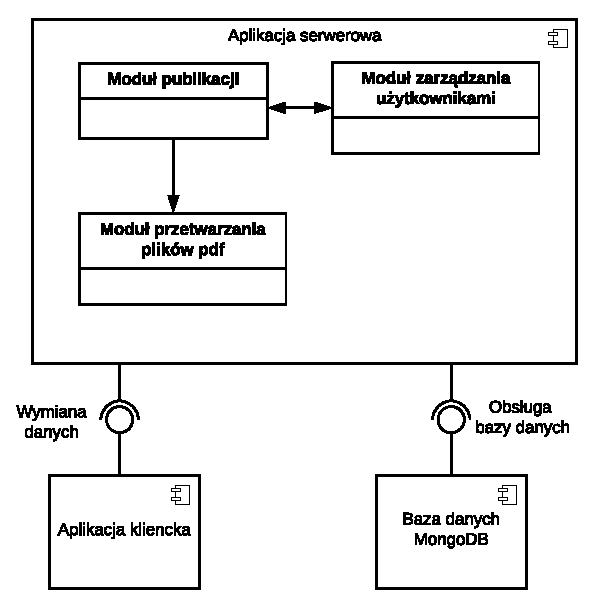
\includegraphics[scale=1.2]{\ImgPath/rys/diag_komp_ogolny.pdf}
 	\end{center}
 	\caption{Ogólna architektura systemu}
 	\label{ogolnaArchitektura}
 \end{figure}
 Przedstawiona na powyższym diagramie aplikacja serwerowa oraz baza danych MongoDB będę uruchamiana jako kontenery Dockera, natomiast aplikacja kliencka będzie pracowała na urządzeniach z systemem Android. Wymiana danych pomiędzy tymi aplikacjami będzie odbywała się za pomocą interfejsu programistycznego(API), w sposób szyfrowany przy wykorzystaniu protokółu HTTPS.
 Baza danych będzie działać w wewnętrznej sieci Dockerowej, do której bezpośredni dostęp będzie posiadała jedynie aplikacja serwerowa. 

\section{Architektura aplikacji serwerowej}
\subsection{Struktura}
Aplikacja serwerowa zbudowana będzie w oparciu o środowisko Node.js. Składać się będzie z 3 podstawowe modułów:
\begin{enumerate}
	\item Moduł zarządzania użytkownikami - będzie odpowiadał za obsługę żądań HTTP dotyczących rejestracji i logowania użytkowników oraz zarządzaniu sesją
	
	\item Moduł publikacji - będzie posiadał następujące zadania:
	\begin{itemize}
		\item obsługa żądań HTTP dotyczących publikacji
		\item zapis, odczyt i modyfikacja publikacji w bazie danych
		\item zlecanie operacji przetwarzania pliku PDF
		\item zapisywanie i odczyt plików PDF przypisanych do publikacji
	\end{itemize}
	 
	\item Moduł przetwarzania plików pdf - jako jedyny nie będzie odpowiadał za obsługę żądań, a za przetwarzania plików pdf. Do przetwarzania plików pdf zostanie wykorzystana biblioteka \textit{pdf-parse}. Będzie dostarczał następujące funkcjonalności:
	\begin{itemize}
		\item odczyt informacji takich jak tytuł lub autor publikacji z metadanych plików PDF
		\item wyszukiwanie DOI w metadanych pliku PDF, bądź w jego treści
		\item pobieranie szczegółów dotyczących przetwarzanej publikacji na podstawie znalezionego wcześniej numery DOI
	\end{itemize}
\end{enumerate}


Dodatkowo żądania HTTP będą przetwarzane wstępnie, także przez następujące moduły pośredniczące:
\begin{enumerate}
	\item Moduł autoryzacyjny - jego rolą będzie sprawdzanie czy dane żądanie wysłane została przez użytkownika, który posiada uprawnienia do jego wykonania
	\item Moduł walidacji danych - będzie odpowiedzialny za sprawdzania czy dane przychodzące w żądaniach, typu POST oraz PUT, które tworzą lub modyfikują informacje w bazie danych, są w odpowiednim formacie
\end{enumerate}


\subsection{Środowisko}
Aplikacja serwerowa będzie przygotowana do pracy jako kontener Dockera. Dzięki temu przy wdrażaniu aplikacji konfiguracja środowiska produkcyjnego, nie będzie wymagała pełnego przygotowania środowiska Node.js, potrzebując do pracy jednie aplikacji Docker oraz docker-compose, która pozwala na zarządzanie i konfigurację wielu kontenerów, mogących współpracować między sobą. Dzięki temu, że baza danych MongoDB może również działać w formie kontenera Dockerowego, przy wykorzystaniu aplikacji docker-compose, uruchomienie całej aplikacji serwerowej wraz bazą danych będzie ograniczać się do pobrania kontenerów oraz ich uruchomienia za pomocą jednego polecenia, a dodatkowo pozwala na wdrożenie aplikacji zarówno przy użyciu systemu Linux i Windows jaki i MacOs.

\section{Architektura aplikacji klienckiej}
Aplikacja kliencka będzie przeznaczona na urządzenia mobilne z systemem Android. Zostanie wykonana w sposób natywny dla tej platformy przy wykorzystaniu środowiska Android Studio oraz języka Kotlin. Zgodnie z zaleceniami występującymi w dokumentacji Android, wykorzystany zostanie uproszczony wzorzec Model–view–viewmodel(MVVM). 

\subsection{Wzorzec Model–view–viewmodel(MVVM)}
Wzorzec MVVM bazuje na popularnym wzorcu Model-view-controller. Jest często wykorzystywany podczas tworzenia aplikacji z interfejsem graficznym, do których możemy zaliczyć programy przeznaczone na system Android. 
Zgodnie z tą architekturą aplikacja składa się z głównych elementów:
\begin{enumerate}
	\item model - przechowuje dane, pobrane przez viewmodel, później prezentowane w warstwie view, nie powinien zawierać logiki biznesowej
	\item view - jest to reprezentacja graficznego widoku, widzianego przez użytkownika aplikacji
	\item viewmodel - element spajający model i view, pod pewnym względem odpowiadający dla wartswy controller z wzorca MVC. Jest odpowiedzialny za wypełnianie widoku danymi, pobranymi z modelu oraz za obsługę interakcji w użytkownikiem. 
\end{enumerate}

Jedną z podstawowych cech tego wzorca jest tak zwany databinding. Polega on automatycznym odświeżaniu danych pochodzących z modelu w widoku, w momencie gdy dojdzie do ich modyfikacji w viewmodelu. Dzięki temu, programista jest zwolniony z ciągłego dbania o uaktualnianie danych prezentowanych w widoku.

\newpage
\subsection{Struktura}
Natywne aplikacje działające pod kontrolą systemu Android zbudowaną są z komponentów zwanych aktywnościami(Activity). Zgodnie z definicją dostępną w dokumentacji, jest to  pojedyncza konkretna czynność, która może zostać wykonana przez użytkownika. Dodatkowo aktywności mogą składać się z mniejszych części zwanych fragmentami. Aplikacja kliencka przygotowywana w ramach tej pracy, będzie składała się z trzech aktywności:
\begin{enumerate}
	\item LoginActivity - aktywność odpowiedzialna za proces logowania użytkownika.
	
	\item MainActivity - główna aktywność służąca do prezentacji listy publikacji danego użytkownika. 

	\item PublicationDetailsActivity - aktywność w której dodaje się nowe publikacje oraz odczytuje i edytuje istniejące.

\end{enumerate}

Do komunikacji z aplikacja serwerową za pomocą protokołu HTTP wykorzystana zostanie biblioteka Retrofit. Wykorzystywana będzie w klasach należących do paczki \textit{network}, która odpowiadać za obsługę żądań HTTP wykorzystywanych do logowania użytkowników oraz do odczytywania, dodawania i edycji publikacji naukowych. 

Do obsługi asynchroniczności zapytań, wszystkie klasy korzystające z paczki \textit{network}, będą wymagały zaimplementowania interfejsu \textit{RequestObserver}, który będzie zawierał dwie metody:
\begin{enumerate}
	\item onSuccess - metoda wywoływana, w przypadku gdy żądanie zakończyło się pomyślnie.
	
	\item onFail - metoda wywoływana, w przypadku gdy żądanie zakończyło się błędem.
\end{enumerate}
\chapter{Szczegóły implementacyjne aplikacji}
\section{Aplikacja serwerowa}
Zgodnie z przedstawioną w poprzednim rozdziale architekturą aplikacji serwerowej została ona podzielona na trzy moduły. W tym rozdziale zostaną przedstawione ich szczegóły implementacyjne oraz sposób komunikacji pomiędzy sobą. Organizacja kodu aplikacji serwerwoej została przedstawiona, na poniższym diagramie klas:

 \begin{figure}[!htbp]
	\begin{center}
		\centering
		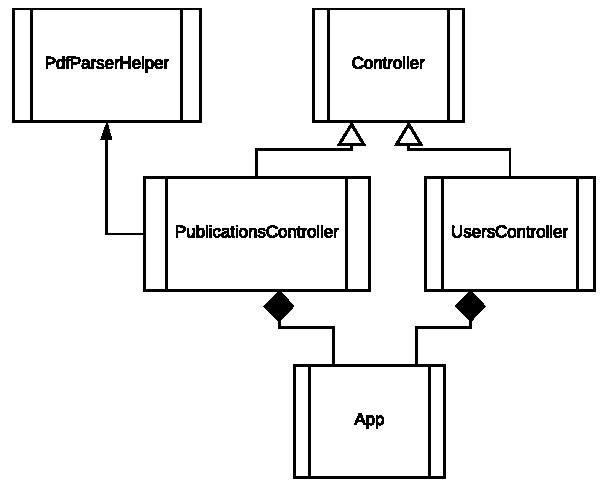
\includegraphics[scale=0.91]{\ImgPath/rys/diag_klas_serwer.pdf}
	\end{center}
	\caption{Diagram klas}
	\label{diagramKlas}
\end{figure}
\subsection{Opis podstawowych klas}
Przedstawione na powyższym diagramie klasy pełnią następujące funkcje:
\begin{enumerate}
	\item App - główna klasa aplikacji, która inicjalizuje wszystkie klasy rozszerzające klasę Controller, a także odpowiedzialna za skonfigurowanie oprogramowania pośredniczącego(middleware) .
	
	\item Controller - klasa rozszerzana przez inne klasy, odpowiedzialne za obsługę żądań  HTTP.
	
	\item UsersController - klasa obsługująca żądania dotyczące rejestracji, logowania, oraz wylogowywania użytkowników.
	
	\item PublicationsController - klasa obsługująca żądania dotyczące dodawania, odczytywania, usuwania oraz edycji publikacji.
	
\end{enumerate}

\section{Obsługa użytkowników}
Cała obsługa użytkowników w systemie została napisana od podstaw. Odpowiedzialna jest za to klasa \textit{UsersController}, odpowiadająca za proces rejestracji i logowania użytkowników oraz oprogramowanie pośredniczące \textit{authMiddleware}, którego zadaniem jest sprawdzanie czy dane żądanie jest wykonywane przez zalogowanego użytkownika, który posiada wystarczające uprawnienia. Do zapewnienia bezpiecznego przechowywania hasła wykorzystana została biblioteka \textit{bcrypt}, za pomocą której uzyskiwana jest sól, wykorzystywana podczas obliczania funkcji skrótu dla hasła. 

Dla celów autoryzacji, dokumenty reprezentujące użytkowników, które przechowywane są w bazie danych, posiadają w swojej strukturze dwa pola:
\begin{itemize}
	\item email - służący do identyfikacji, użytkownika, który próbuje zalogować się do systemu
	
	\item hash - pole zawierające sól oraz wynik funkcji skrótu dla hasła danego użytkownika
	
\end{itemize}
Dzięki przechowywaniu wyniku funkcji skrótu dla hasła, zamiast jawnego jego przechowywania, podnoszony jest poziom bezpieczeństwa. Nawet w przypadku, gdy dane z bazy danych zostaną wykradzione, hasła użytkowników systemu nie będą mogły zostać odczytane. Wynika to z własności funkcji skrótu, które nie pozwala w łatwy sposób odczytać wartości wejściowej, nawet przy posiadania soli, która została wykorzystana podczas obliczania wyniku funkcji.

\newpage
\subsection{Proces rejestracji użytkownika}

Proces rejestracji użytkownika posiada następujący przebieg:
 \begin{figure}[!htbp]
	\begin{center}
		\centering
		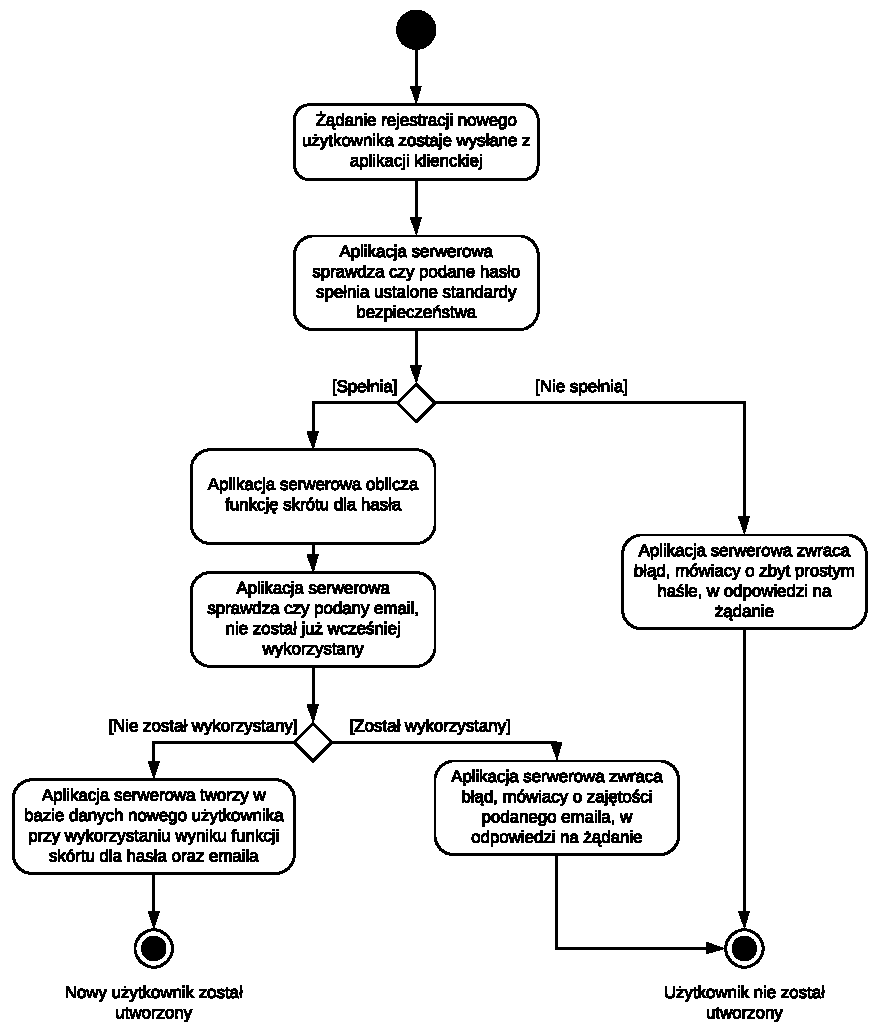
\includegraphics[scale=1]{\ImgPath/rys/diag_aktyw_rejestr.pdf}
	\end{center}
	\caption{Diagram aktywności dla procesu rejestracji}
	\label{diagramAktywnosciRejstracja}
\end{figure}

\subsection{Proces logowania użytkownika}

\begin{thebibliography}{99}
\addcontentsline{toc}{chapter}{Bibliografia}
\bibitem{LOKI2}{daemon9, ,,LOKI2'', Phrack Magazine, Issue 51. 
\url{http://phrack.org}}
\bibitem{RWWWS}{van Hauser, Reverse WWW Shell,  THC, The Hacker's 
Choice.\newline \url{www.thc.org}}


\end{thebibliography}

\zakonczenie  % wklejenie recenzji i opinii

\end{document}
%+++ END +++
